\subsection{Arquitectura del sistema}

La proposta combina components executats dins del navegador, serveis locals d'anàlisi i fonts externes vinculades a l'ecosistema Web3. La Figura~\ref{fig:visio_general} delimita aquest context i mostra com l'usuari, les interfícies d'origen i la xarxa blockchain es relacionen amb l'entorn local que conté MetaMask, el Snap, el backend, el model de llenguatge local i la base de dades local.

\begin{figure}[H]
\centering
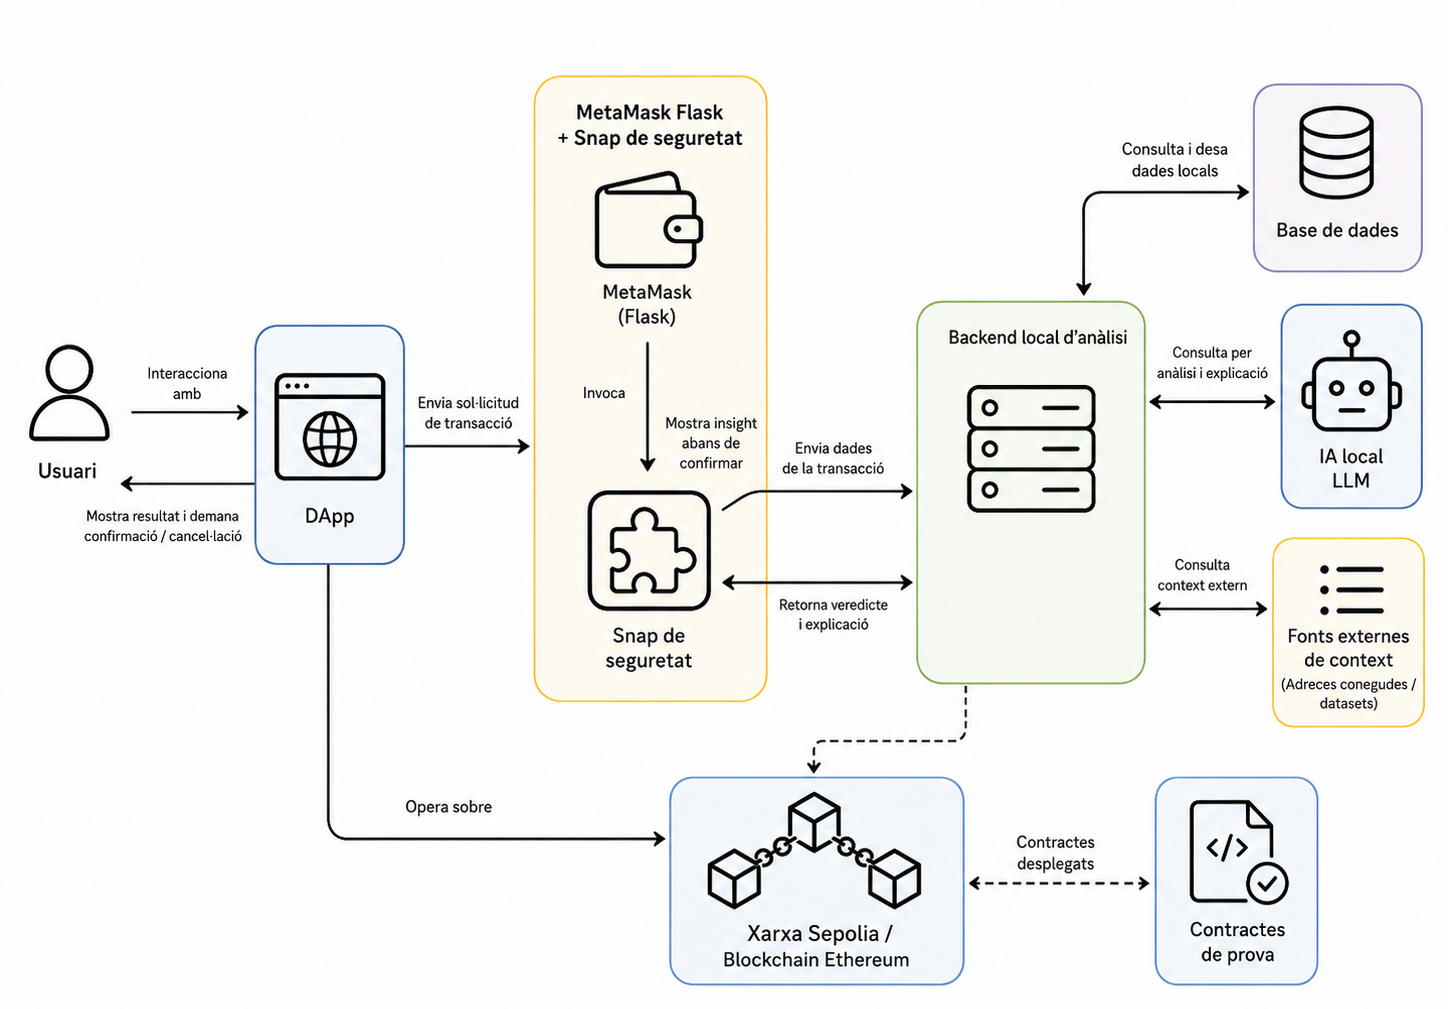
\includegraphics[width=\textwidth]{imgs/arquitectura_general_final.png}
\caption{Visió general del sistema d’assistència abans de la confirmació d’una transacció}
\label{fig:visio_general}
\end{figure}

\noindent\textbf{Flux resumit}

Tal com mostra la Figura~\ref{fig:visio_general}, el flux comença quan l’usuari interactua amb una DApp i aquesta sol·licita una transacció a MetaMask. Abans de presentar-ne la confirmació definitiva, MetaMask activa el Snap mitjançant el punt d’entrada \texttt{onTransaction}. El Snap recull les dades disponibles de l’operació, les prepara en un format coherent i les envia al \textit{backend} local perquè en faci l’anàlisi.

Un cop rebuda la sol·licitud, el \textit{backend} normalitza i descodifica la transacció, aplica les regles deterministes i consulta, quan és necessari, el context disponible. Aquest context combina la informació \textit{on-chain} amb les adreces conegudes, els conjunts de dades externs i la memòria d’anàlisis anteriors emmagatzemada a la base de dades local. A continuació, el model de llenguatge aporta una revisió i una explicació en llenguatge natural, sempre subordinades als fets verificats pel motor determinista. Amb tots aquests elements, el \textit{backend} construeix el veredicte final i el retorna al Snap.

Finalment, el Snap adapta la resposta al format admès per MetaMask i mostra l’\textit{insight} de seguretat abans que l’usuari prengui la decisió. D’aquesta manera, la persona pot revisar el nivell de risc, els motius detectats i les conseqüències principals de l’operació abans de confirmar-la o cancel·lar-la. La mateixa arquitectura permet conservar el resultat per enriquir anàlisis posteriors sense alterar el paper de MetaMask com a punt final de decisió.



\subsubsection{Flux de comunicació}

Després de delimitar els components i les seves responsabilitats en la visió general, la Figura~\ref{fig:flux_complet_seq} presenta l'ordre temporal de la comunicació, des de la sol·licitud inicial fins a la decisió de l'usuari.

\begin{figure}[H]
\centering
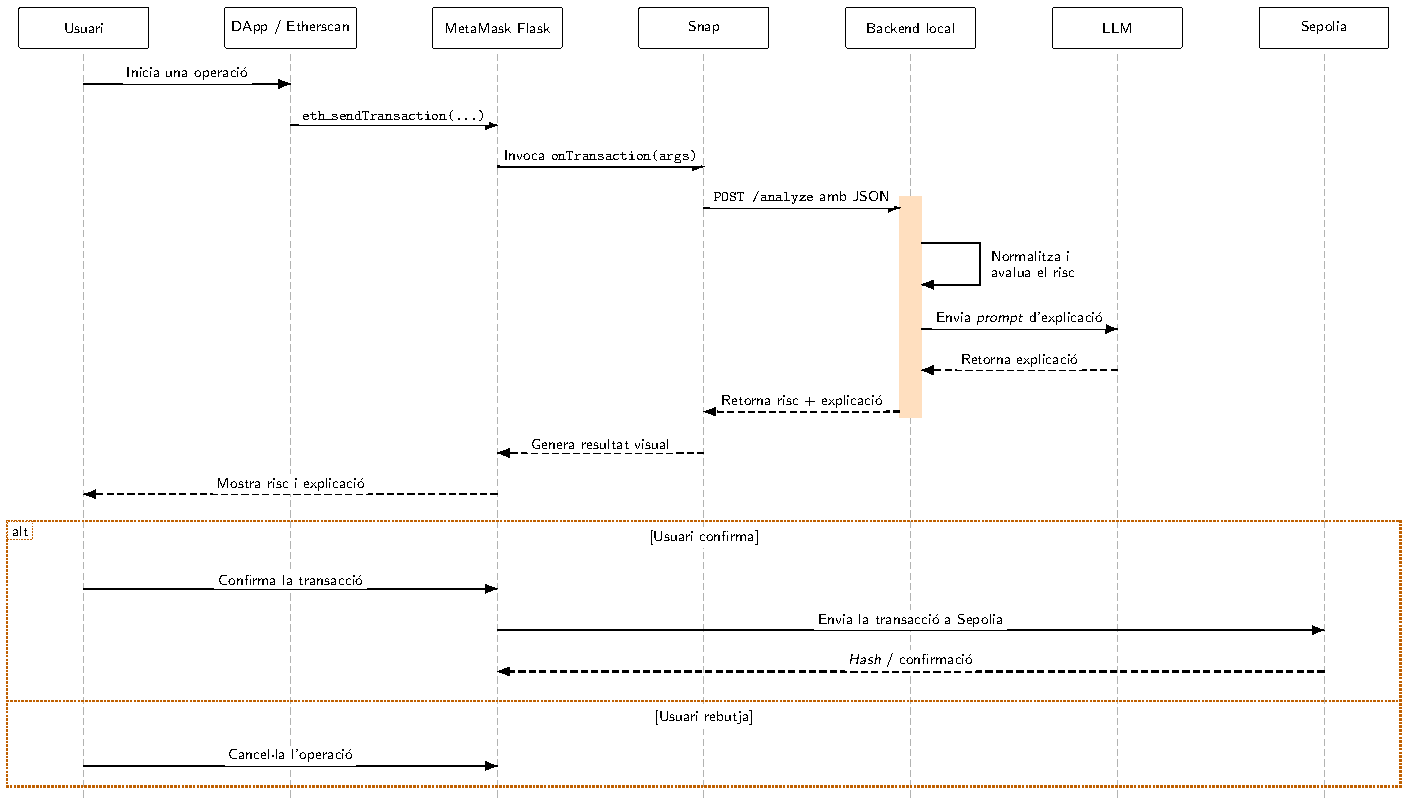
\includegraphics[width=\textwidth]{diagrams/render_sequence_flux_complet.pdf}
\caption{Flux complet d'execució del prototip, des de la generació de la transacció fins a la decisió final de l'usuari}
\label{fig:flux_complet_seq}
\end{figure}
